Certyfikaty SSL to niewielkie pliki danych, które w sposób cyfrowy wiążą klucz kryptograficzny z danymi organizacji. Po zainstalowaniu na serwerze WWW, aktywuje on kłódkę i protokół https oraz umożliwia bezpieczne połączenia z serwera WWW do przeglądarki. Zazwyczaj SSL jest używany do zabezpieczania transakcji kartami kredytowymi, przesyłania danych i logowania, a ostatnio staje się normą przy zabezpieczaniu przeglądania stron serwisów społecznościowych.
Do naszych celów certyfikat został wygenerowany dzięki darmowemu urządowi certyfikacji Let's Encrypt (rys. \ref{fig:ssl})

\begin{figure}[H]
    \centering
    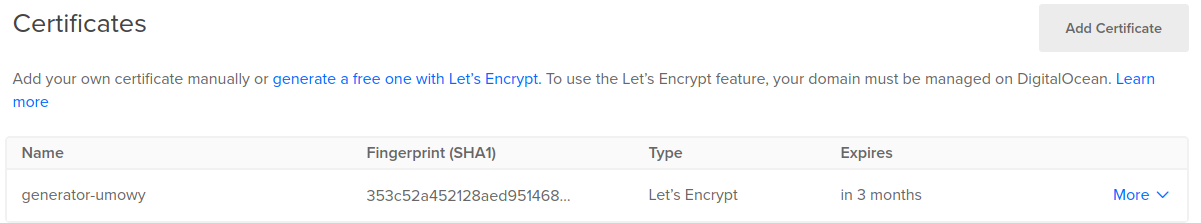
\includegraphics[width=6in]{images/ssl.png}
    \caption{Przykład dodania certyfikatu na stronie https://cloud.digitalocean.com \label{fig:ssl}}
\end{figure}